\section{Elastisk net}
I dette afsnit introduceres en shrinkage metode kaldet elastisk net, som kombinerer ridge regression og lasso.
Metoden blev først præsenteret i \citep{zou_hastie}.

Selvom lasso har vist succes i mange tilfælde, har den også nogle begrænsninger:
%
\begin{enumerate}[label=\textnormal{(\arabic*)}]
    \item Hvis $p>n$, da udvælger lasso højst $n$ variable, som følge af at lasso er et konveks optimeringsproblem. Derudover er lasso ikke veldefineret medmindre \(\Vert \beta \Vert_1 \leq t\). \label{itm:1}
    \item Hvis der eksisterer en gruppe af variable, som har høj parvis korrelation, da har lasso en tendens til blot at udvælge  én variabel fra denne gruppe og denne variabel udvælges tilfældigt. \label{itm:2}
    \item Hvis $n>p$ og variablerne er højt korreleret, da er det empirisk bevist, at lasso prædikterer dårligere end ridge regression \citep{lasso}.  \label{itm:3}
\end{enumerate}
%
Målet er at finde en metode, som overkommer ovenstående begrænsninger.
%
\begin{defn}[Naiv elastisk net]
Naive elastiske net løser følgende optimeringsproblem
\begin{align}
\widehat{\tbeta}^\text{naivEN} = \argmin_{\tbeta} \cbr{\Vert \y - \X \tbeta \Vert_2^2 + \lambda_2 \Vert \tbeta \Vert_2^2 + \lambda_1 \Vert \tbeta \Vert_1}, \label{eq:naivEN}
\end{align}
for \(\lambda_1, \lambda_2 \geq 0\).
\end{defn}
%
Lad \(\alpha = \frac{\lambda_1}{\lambda_1 + \lambda_2}\), da er \eqref{eq:naivEN} ækvivalent med optimeringsproblemet
\begin{align*}
\widehat{\tbeta}^\text{naivEN} = \argmin_{\tbeta} \cbr{\Vert \y - \X \tbeta \Vert_2^2}, \ \text{underlagt at } \frac{1}{2}\del{1-\alpha} \Vert \tbeta \Vert_2^2 + \alpha \Vert \tbeta \Vert_1 \leq t,
\end{align*}
som kan omskrives til et Lagrange problem
\begin{align}
\widehat{\tbeta}^\text{naivEN} =\argmin_{\tbeta} \cbr{ \Vert \y - \X \tbeta \Vert_2^2 + \lambda \sbr{\frac{1}{2}(1- \alpha) \Vert \tbeta \Vert_2^2 + \alpha \Vert \tbeta \Vert_1}}. \label{eq:4.2}
\end{align}
Hvis $\alpha=0$, da reduceres det til den kvadrerede $\ell_2$-norm svarende til strafleddet for ridge regression, og hvis $\alpha=1$ reduceres strafleddet til $\ell_1$-normen svarende til strafleddet for lasso.
Optimeringsproblemet  \eqref{eq:4.2} er streng konveks for \(\alpha \in [0,1)\), hvilket betyder, at der eksisterer en entydig løsning uafhængigt af korrelationsstrukturen af $\X$.
For  \(\alpha=1\) er problemet konveks, men ikke streng konveks.
Dette ses tydeligt på figur \ref{fig:elastisk}.
%
\begin{figure}[H]
\centering
\scalebox{0.8}{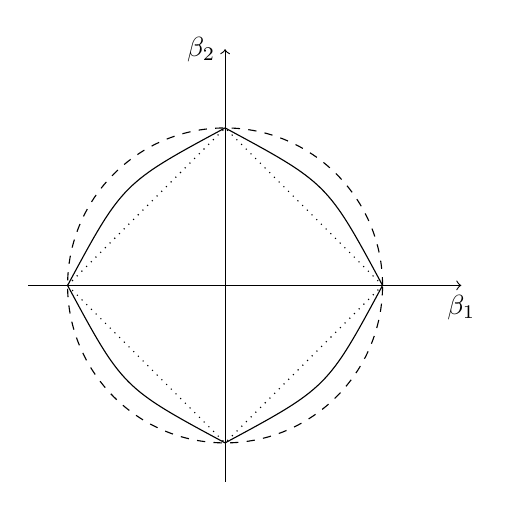
\begin{tikzpicture}
\draw[dashed] (0,0) circle (2cm);
\draw[dotted] (-2,0) -- (0,-2) -- (2,0) -- (0,2) -- (-2,0); 
\draw (-2,0) .. controls (-1.3,1.3) .. (0,2);
\draw (0,2) .. controls (1.3,1.3) .. (2,0);
\draw (-2,0) .. controls (-1.3,-1.3) .. (0,-2);
\draw (0,-2) .. controls (1.3,-1.3) .. (2,0);
\draw [<-] (0,3) node [left] {$\beta_2$}-- (0,-2.5);
\draw[<-] (3,0) node [below] {$\beta_1$} -- (-2.5,0);
\end{tikzpicture}}
\caption[optional short text]{Betingelsesområderne for ridge regression (\tikz[baseline]{\draw[dashed] (0,.5ex)--++(.5,0) ;}), lasso (\tikz[baseline]{\draw[dotted] (0,.5ex)--++(.5,0) ;}) og elastisk net med \(\alpha = 0.5\) (\tikz[baseline]{\draw (0,.5ex)--++(.5,0) ;}) i to dimensioner. Vi observerer, at singulariteter i hjørnerne og kanterne er streng konveks. Styrken af konveksitet varierer med \(\alpha\).} \label{fig:elastisk}
\end{figure}
%
%\imgfigh{crime_el_lasso.pdf}{0.7}{Koefficientstierne for henholdsvis lasso og elastisk net med \(\alpha=0.3\) plottet imod log af $\lambda$ for crime data.}{crime_el_lasso}
%
%\begin{figure}[H]
%\centering
%\begin{minipage}{0.4\linewidth}
%\scalebox{0.32}{\includegraphics{fig/img/crime_lasso.png}}
%\end{minipage}
%\hspace{0.2cm}
%\begin{minipage}{0.4\linewidth}
%\scalebox{0.32}{\includegraphics{fig/crime_EN.png}}
%\end{minipage}
%\caption{Koefficientstierne for henholdsvis lasso (ventre) og elastisk net med \(\alpha=0.3\) (højre) plottet imod \(\ell_1\)-normen for crime data.} \label{fig:crime_koef_EN}
%\end{figure}
%
%En tre dimensionel illustration af betingelsesområderne for det elastiske net og standard lasso er givet på figur \ref{fig:elastisk_net}.
%Heraf ses at det elastiske net har egenskaberne af både $\ell_1$ kuglen og $\ell_2$ kuglen: de skarpe hjørner og kanter opfordrer til variable udvælgelse, mens de kurvede konturer opfordrer stærk korreleret variable til at dele koefficienter.
%%
%\begin{figure}[H]
%\centering
% \scalebox{0.5}{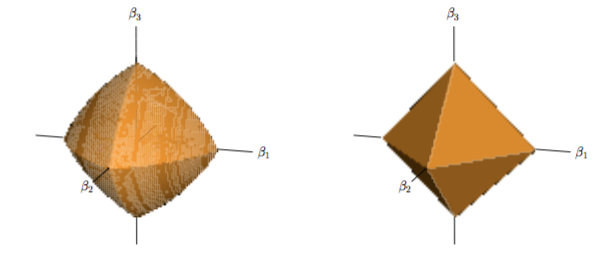
\includegraphics{fig/elastisk_net.jpg}}
%\caption{Kuglen for elastisk net med \(\alpha=0.7\) (venstre) og \(\ell_1\) kuglen (højre) i tre dimensioner.}
%\label{fig:elastisk_net}
%\end{figure}
%
Det viser sig, at optimeringsproblemet for naiv elastisk net kan transformeres til et ækvivalent lasso problem på augmented data.
%
\begin{lem} \label{lem:elastisk_net}
Givet data \(\del{\y, \X}\) og parametrene \(\del{\lambda_1, \lambda_2}\), defineres et augmented datasæt 
\begin{align*}
\X^* = \del{1 + \lambda_2}^{-1/2} \begin{pmatrix}
\X \\ \sqrt{\lambda_2} \mathbf{I}_p
\end{pmatrix}, \quad \y^* = \begin{pmatrix}
\y \\ \mathbf{0}
\end{pmatrix},
\end{align*}
hvor \(\X^*\) er en \(\del{n+p} \times p\) matrix og \(\y^*\) er en \(n + p\) vektor. 
Lad \(\gamma = \frac{\lambda_1}{\sqrt{1+\lambda_2}}\) og \(\tbeta^* = \sqrt{1+\lambda_2} \tbeta^\text{naivEN}\), da kan \eqref{eq:naivEN} omskrives til
\begin{align}
\widehat{\tbeta}^* = \argmin_{\tbeta^*} \cbr{ \Vert \y^* - \X^* \tbeta^* \Vert_2^2 +\gamma \Vert \tbeta^* \Vert_1}, \label{eq:EN11}
\end{align}
hvor
\begin{align*}
\widehat{\tbeta}^\text{naivEN} = \frac{1}{\sqrt{1+\lambda_2}} \widehat{\tbeta}^*.
\end{align*}
\end{lem}
%
\begin{proof}
Vi har, at
\begin{align*}
\widehat{\tbeta}^\text{naivEN} = \frac{1}{\sqrt{1+\lambda_2}} \widehat{\tbeta}^*,
\end{align*}
hvor \(\widehat{\tbeta}^*\) er givet i \eqref{eq:EN11}, således får vi, at
\begin{align*}
\widehat{\tbeta}^\text{naivEN} &= \argmin_{\tbeta} \cbr{ \left\Vert \begin{pmatrix}
\y \\ \mathbf{0}
\end{pmatrix} -  \del{1 + \lambda_2}^{-1/2} \begin{pmatrix}
\X \\ \sqrt{\lambda_2} \mathbf{I}_p
\end{pmatrix} \sqrt{1+\lambda_2} \tbeta \right\Vert_2^2 + \frac{\lambda_1}{\sqrt{1+\lambda_2}} \left\Vert \sqrt{1+\lambda_2} \tbeta \right\Vert_1} \\
&= \argmin_{\tbeta} \cbr{ \left\Vert \begin{pmatrix}
\y \\ \mathbf{0}
\end{pmatrix} -  \begin{pmatrix}
\X \\ \sqrt{\lambda_2} \mathbf{I}_p
\end{pmatrix} \tbeta \right\Vert_2^2 + \lambda_1 \left\Vert \tbeta \right\Vert_1} \\
&= \argmin_{\tbeta} \cbr{ \left\Vert \begin{pmatrix}
\y - \X \tbeta \\ - \sqrt{\lambda_2} \tbeta 
\end{pmatrix} \right\Vert_2^2 + \lambda_1 \left\Vert \tbeta \right\Vert_1} \\
 &= \argmin_{\tbeta} \cbr{ \Vert \y - \X \tbeta \Vert_2^2 + \lambda_2 \Vert \tbeta \Vert_2^2 + \lambda_1 \Vert \tbeta \Vert_1}.
\end{align*}
\end{proof}
%Beviset følger af simpel algebra og er derfor undladt.
Naiv elastisk net kan i princippet vælge alle \(p\) prædiktorer i alle tilfælde, da \(\X^*\) har rang \(p\).
Dermed er naiv elastisk net ikke begrænset til blot at vælge \(n\) prædiktorer, hvis \(p > n\), som er tilfældet for lasso som beskrevet i punkt \ref{itm:1}.
Lemma \ref{lem:elastisk_net} viser også, at naiv  elastisk net udfører variabeludvælgelse svarende til lasso.
%
\begin{lem}
Hvis \(\X\) er ortogonal, da gælder, at
\begin{align}
\widehat{\beta}_j^\text{ridge} &= \frac{\widehat{\beta}_j^\text{OLS}}{1+\lambda_2}, \label{eq:orto_ridge} \\
\widehat{\beta}_j^\text{lasso} &= \text{sign} \del{\widehat{\beta}_j^\text{OLS}} \del{\left\vert \widehat{\beta}_j^\text{OLS} \right\vert - \frac{\lambda_1}{2}}_+ =S_{\frac{\lambda_1}{2}} \del{ \widehat{\beta}_j^\text{OLS}}, \label{eq:orto_lasso} \\
\widehat{\beta}_j^\text{naivEN} &= \text{sign} \del{\widehat{\beta}_j^\text{OLS}} \frac{\del{\left\vert \widehat{\beta}_j^\text{OLS} \right\vert - \frac{\lambda_1}{2}}_+}{1+\lambda_2} = \frac{S_{\frac{\lambda_1}{2}} \del{ \widehat{\beta}_j^\text{OLS}} }{1+\lambda_2} . \label{eq:orto_naivEN}
\end{align}
Hvis \(\X\) er ortogonal, illustrerer figur \ref{fig:elastisk2} en sammenligning af ridge regression, lasso og naiv elastisk net.
Heraf ses det også at naiv elastisk net er en to-trins procedure, først mindskes koefficienterne udfra ridge regression, hvorefter lasso udfører variabeludvælgelse. 
%har vi en ridge lignende shrinkage, som efterfølges af en lasso lignende thresholding.
%
\begin{figure}[H]
\centering
\scalebox{0.8}{\begin{tikzpicture}
\draw[loosely dotted] (-3,-3) -- (3,3);
\draw[dotted] (-3,-2) -- (3,2);
\draw (-3,-1.5) -- (-0.75,0) -- (0.75,0) -- (3,1.5);
\draw[dashed] (-3,-2.2) -- (-0.75,0) -- (0.75,0) -- (3,2.2); 
\draw [<-] (0,3.5) node [left] {$\widehat{\beta}$}-- (0,-3.5);
\draw[<-] (3.5,0) node [below] {$\beta$} -- (-3.5,0);
\end{tikzpicture}
}
\caption[optional short text]{Eksakte løsninger for ridge regression (\tikz[baseline]{\draw[dotted] (0,.5ex)--++(.5,0) ;}), lasso (\tikz[baseline]{\draw[dashed] (0,.5ex)--++(.5,0) ;}) og naiv elastisk net (\tikz[baseline]{\draw (0,.5ex)--++(.5,0) ;}), hvis \(\X\) er ortogonal (\tikz[baseline]{\draw[loosely dotted] (0,.5ex)--++(.5,0) ;} OLS) for parametrene \(\lambda_1=2\) og \(\lambda_2=1\).} \label{fig:elastisk2}
\end{figure}
%
\end{lem}
%
\begin{proof}
Estimatoren for ridge regression i det ortogonale tilfælde \eqref{eq:orto_ridge} følger direkte udfra ridge estimatoren \eqref{eq:ridge_estimator}, da \(\X^T \X = \mathbf{I}_p\) og \(\widehat{\tbeta}^\text{OLS} = \X^T \y\).
For at bevise lasso estimatoren i det ortogonale tilfælde \eqref{eq:orto_lasso}, omskrives lasso problemet \eqref{eq:2.5} til følgende
\begin{align*}
\widehat{\tbeta}^\text{lasso} &= \argmin_{\tbeta} \cbr{\del{\y - \X \tbeta}^T \del{\y - \X \tbeta} + \lambda_1 \Vert \tbeta \Vert_1} \\
&= \argmin_{\tbeta} \cbr{ \y^T \y - 2 \tbeta^T \X^T \y + \tbeta^T \X^T \X \tbeta + \lambda_1 \Vert \tbeta \Vert_1} \\
&= \argmin_{\tbeta} \cbr{- 2 \tbeta^T \widehat{\tbeta}^\text{OLS} + \tbeta^T \tbeta + \lambda_1 \Vert \tbeta \Vert_1}.
\end{align*}
Lad os blot betragte \(j\)'te indeks af lasso estimatoren
\begin{align*}
\widehat{\beta}_j^\text{lasso} = \argmin_{\beta_j} \cbr{ - 2 \beta_j \widehat{\beta}_j^\text{OLS} + \beta_j^2 + \lambda_1 \vert \beta_j \vert}.
\end{align*}
Vi differentierer
\begin{align*}
\frac{\partial}{\partial \beta_j} \del{- 2 \beta_j \widehat{\beta}_j^\text{OLS} + \beta_j^2 + \lambda_1 \vert \beta_j \vert}
=-2\widehat{\beta}^\text{OLS} + 2\beta_j + \begin{cases}
-\lambda_1 \quad &\beta_j < 0 \\
[-\lambda_1, \lambda_1] & \beta_j = 0 \\
\lambda_1 & \beta_j >0 
\end{cases},
\end{align*}
dette sættes lig \(0\) og isolerer for \(\beta_j\)
\begin{align*}
\widehat{\beta}_j^\text{lasso} &= \widehat{\beta}_j^\text{OLS} - \frac{1}{2}\begin{cases}
-\lambda_1 \quad &\beta_j < 0 \\
[-\lambda_1, \lambda_1] & \beta_j = 0 \\
\lambda_1 & \beta_j >0 
\end{cases} \\
&= \begin{cases}
\widehat{\beta}_j^\text{OLS} + \frac{\lambda_1,}{2} \quad &\widehat{\beta}_j^\text{OLS} < - \frac{\lambda_1}{2} \\
0, &\left\vert\widehat{\beta}_j^\text{OLS} \right\vert \leq \frac{\lambda_1}{2} \\
\widehat{\beta}_j^\text{OLS} - \frac{\lambda_1}{2}, \quad &\widehat{\beta}_j^\text{OLS} > \frac{\lambda_1}{2}
\end{cases}. 
\end{align*}
Hvoraf vi får, at \(\widehat{\beta}_j^\text{lasso} = S_{\frac{\lambda_1}{2}} \del{ \widehat{\beta}_j^\text{OLS}} \), som fuldfører beviset.
Estimatoren for naiv elastisk net i det ortogonale tilfælde \eqref{eq:orto_naivEN} følger af \eqref{eq:orto_ridge} og \eqref{eq:orto_lasso}, da denne er en kombination heraf.
\end{proof}
%
Hvis vi har en gruppe af højt korreleret variable, da vil lasso blot udvælge én variabel og den udvælges tilfældigt, som nævnt i punkt \ref{itm:2}.
Men naiv elastisk net udvælger alle variable i denne gruppe, som vi nu vil vise. 
En regressionsmetode udviser denne evne, hvis regressionskoeffcienterne af en gruppe af højt korreleret variable er approksimativt ens.
%
\begin{lem} \label{lem:elastisk_net2}
Lad os betragte
\begin{align}
\widehat{\tbeta} = \argmin_{\tbeta} \Vert \y - \X \tbeta \Vert_2^2 + \lambda J \del{\tbeta}, \label{eq:EN10}
\end{align}
hvor \(J \del{\cdot}\) er positiv for \(\tbeta \neq 0\).
Antag \(\x_i = \x_j\), for \(i, j = 1, \ldots, p\).
\begin{enumerate}[label=\alph*)]
\item Hvis \(J \del{\cdot}\) er streng konveks, da er \(\widehat{\beta}_i = \widehat{\beta}_j\), for alle \(\lambda \geq 0\).
\item Hvis \(J \del{\tbeta} = \Vert \tbeta \Vert_1\), da er \(\widehat{\beta}_i \widehat{\beta}_j \geq 0\) og \(\widehat{\tbeta}^*\) er optimum af \eqref{eq:EN10}, hvor
\begin{align*}
\widehat{\beta}_k^* = \begin{cases}
\widehat{\beta}_k & k \neq i \text{ og } k \neq j, \\
\del{\widehat{\beta}_i + \widehat{\beta}_j} s & k = i, \\
\del{\widehat{\beta}_i + \widehat{\beta}_j} \del{1-s} & k = j,
\end{cases}
\end{align*}
for ethvert \(s \in \sbr{0,1}\).
\end{enumerate}
\end{lem}
%
\begin{proof}
Først bevises a).
Fasthold \(\lambda > 0\).
Hvis \(\widehat{\beta}_i \neq \widehat{\beta}_j\), lad os betragte \(\widehat{\tbeta}^*\) som
\begin{align*}
\widehat{\beta}_k^* = \begin{cases}
\widehat{\beta}_k & k \neq i \text{ og } k \neq j, \\
\frac{1}{2} \del{\widehat{\beta}_i + \widehat{\beta}_j} & k = i \text{ eller } k = j.
\end{cases}
\end{align*}
Da \(\x_i = \x_j\), må vi have at \(\X \widehat{\tbeta}^* = \X \widehat{\tbeta}\) og dermed \(\Vert \y - \X \widehat{\tbeta}^* \Vert_2^2 = \Vert \y - \X \widehat{\tbeta} \Vert_2^2\).
Men da \(J \del{\cdot}\) er streng konveks, må vi have, at \(J \del{\widehat{\tbeta}^*} < J \del{\widehat{\tbeta}}\).
Dermed kan \(\widehat{\tbeta}\) ikke være optimum af \eqref{eq:EN10}, som er en modstrid, og vi må have at \(\widehat{\beta}_i = \widehat{\beta}_j\).

Herefter bevises b).
Hvis \(\widehat{\beta}_i \widehat{\beta}_j < 0\), lad os igen betragte \(\widehat{\tbeta}^*\) som ovenfor.
Da ser vi, at \(\vert \widehat{\tbeta}^* \vert < \vert \widehat{\tbeta} \vert\), så \(\widehat{\tbeta}\) kan ikke være en lasso løsning, altså må \(\widehat{\beta}_i \widehat{\beta}_j \geq 0\).
MANGLER NOGET!
fra wiki: hvis der er en løsning \(\hat{\tbeta}\) hvor \(\hat{\beta}_j \hat{\beta}_k \geq 0\), da hvis \(s \in \sbr{0,1}\) erstatter \(\hat{\beta}_j\) med \(s (\hat{\beta}_j + \hat{\beta}_k)\) og \(\hat{\beta}_k\) med \( (1-s)(\hat{\beta}_j + \hat{\beta}_k)\), men de resterende \(\hat{\beta}_i\) fastholdes, giver en ny løsn, således at lasso objektfunktion har en række gyldige minimeringer, dvs ikke entydig!!   
\end{proof}
Hvis vi har identiske prædiktorer, da siger lemma \ref{lem:elastisk_net2}, at streng konveksitet sikrer at alle variable i en gruppe vælges.
Elastisk net med \(\lambda_2 > 0\) er streng konveks, og har dermed denne egenskab, som ønsket.
%
\begin{thm} \label{thm:elastisk_net}
Givet data \(\del{\y, \X}\) og parametrene \(\del{\lambda_1, \lambda_2}\), hvor responsvariablen er centreret og prædiktorerne er standardiseret.
Lad \(\widehat{\tbeta}^\text{naivEN} \del{\lambda_1, \lambda_2}\) være estimatet for naiv elastisk net.
Antag \(\widehat{\beta}^\text{naivEN}_i \del{\lambda_1, \lambda_2} \widehat{\beta}^\text{naivEN}_j \del{\lambda_1, \lambda_2} > 0\).
Definer
\begin{align*}
D_{\lambda_1, \lambda_2} \del{i,j} = \frac{1}{\Vert \y \Vert_1} \left\vert \widehat{\beta}^\text{naivEN}_i \del{\lambda_1, \lambda_2} - \widehat{\beta}^\text{naivEN}_j \del{\lambda_1, \lambda_2} \right\vert,
\end{align*}
da er
\begin{align}
D_{\lambda_1, \lambda_2} \del{i,j} \leq \frac{1}{\lambda_2} \sqrt{2 \del{1-\rho}}, \label{eq:EN5}
\end{align}
hvor \(\rho = \mathbf{x}_i^T \mathbf{x}_j\) er den empiriske korrelation.
\end{thm}
%
\begin{proof}
Hvis \(\widehat{\beta}^\text{naivEN}_i \del{\lambda_1, \lambda_2} \widehat{\beta}^\text{naivEN}_j \del{\lambda_1, \lambda_2} > 0\), da er både \(\widehat{\beta}^\text{naivEN}_i \del{\lambda_1, \lambda_2}\) og \(\widehat{\beta}^\text{naivEN}_j \del{\lambda_1, \lambda_2}\) ikke-nul og der må gælder, at \(\text{sign} \cbr{\widehat{\beta}^\text{naivEN}_i \del{\lambda_1, \lambda_2}} = \text{sign} \cbr{\widehat{\beta}^\text{naivEN}_j \del{\lambda_1, \lambda_2}}\).
Lad \(L \del{\lambda_1,\lambda_2, \tbeta} = \Vert \y - \X \tbeta \Vert_2^2 + \lambda_2 \Vert \tbeta \Vert_2^2 + \lambda_1 \Vert \tbeta \Vert_1\), således at \(\arg \min_{\tbeta} \cbr{L \del{\lambda_1,\lambda_2, \tbeta}}\) svarer til \eqref{eq:naivEN}.
Da må \(\widehat{\tbeta}^\text{naivEN} \del{\lambda_1, \lambda_2}\) opfylde, at
\begin{align*}
\frac{\partial L \del{\lambda_1,\lambda_2, \tbeta} }{\partial \beta_k} \Bigr|_{\tbeta = \widehat{\tbeta}^\text{naivEN} \del{\lambda_1, \lambda_2}}=0, \text{ hvis } \widehat{\beta}^\text{naivEN}_k \del{\lambda_1, \lambda_2} \neq 0.
\end{align*}
Derfor har vi, at
\begin{align}
-2 \mathbf{x}_i^T \del{\y - \X \widehat{\tbeta}^\text{naivEN} \del{\lambda_1, \lambda_2}} +  2 \lambda_2 \widehat{\beta}^\text{naivEN}_i \del{\lambda_1, \lambda_2} + \lambda_1 \text{sign} \cbr{\widehat{\beta}^\text{naivEN}_i \del{\lambda_1, \lambda_2}} &= 0, \label{eq:EN2}\\
-2 \mathbf{x}_j^T \del{\y - \X \widehat{\tbeta}^\text{naivEN} \del{\lambda_1, \lambda_2}} + 2 \lambda_2 \widehat{\beta}^\text{naivEN}_j \del{\lambda_1, \lambda_2} + \lambda_1 \text{sign} \cbr{\widehat{\beta}^\text{naivEN}_j \del{\lambda_1, \lambda_2}} &= 0. \label{eq:EN3}
\end{align}
Vi subtraherer \eqref{eq:EN3} fra \eqref{eq:EN2} og finder, at
\begin{align*}
\del{\mathbf{x}_j^T-\mathbf{x}_i^T} \del{\y - \X \widehat{\tbeta}^\text{naivEN} \del{\lambda_1, \lambda_2}} + \lambda_2 \del{\widehat{\beta}^\text{naivEN}_i \del{\lambda_1, \lambda_2} - \widehat{\beta}^\text{naivEN}_j \del{\lambda_1, \lambda_2}} =0,
\end{align*}
som er ækvivalent med
\begin{align}
\widehat{\beta}^\text{naivEN}_i \del{\lambda_1, \lambda_2} - \widehat{\beta}^\text{naivEN}_j \del{\lambda_1, \lambda_2} = \frac{1}{\lambda_2} \del{\mathbf{x}_i^T-\mathbf{x}_j^T} \widehat{\mathbf{r}}\del{\lambda_1, \lambda_2}, \label{eq:EN4}
\end{align}
hvor \(\widehat{\mathbf{r}}\del{\lambda_1, \lambda_2} = \y - \X  \widehat{\tbeta}^\text{naivEN} \del{\lambda_1, \lambda_2}\) er en vektor af residualer.
Da \(\X\) er standardiseret, har vi, at \(\Vert \mathbf{x}_i - \mathbf{x}_j \Vert_2^2=2 \del{1-\rho}\), hvor \(\rho = \mathbf{x}_i^T \mathbf{x}_j\).
Af \eqref{eq:naivEN} må vi have, at
\begin{align*}
L \del{\lambda_1,\lambda_2, \widehat{\tbeta}^\text{naivEN} \del{\lambda_1, \lambda_2}} \leq L \del{\lambda_1,\lambda_2, \tbeta = 0},  
\end{align*}
dvs
\begin{align*}
\left\Vert \widehat{\mathbf{r}} \del{\lambda_1, \lambda_2} \right\Vert_2^2 + \lambda_2 \left\Vert \widehat{\tbeta}^\text{naivEN} \del{\lambda_1, \lambda_2} \right\Vert_2^2 + \lambda_1 \left\Vert \widehat{\tbeta}^\text{naivEN} \del{\lambda_1, \lambda_2} \right\Vert_1 \leq \left\Vert \y \right\Vert_2^2.  
\end{align*}
Dermed er \(\Vert \widehat{\mathbf{r}} \del{\lambda_1, \lambda_2} \Vert_2 \leq \Vert \y \Vert_2\) og \eqref{eq:EN4} medfører, at
\begin{align*}
D_{\lambda_1, \lambda_2} \del{i,j} &= \frac{1}{\Vert \y \Vert_1} \left\vert \frac{1}{\lambda_2} \del{\mathbf{x}_i^T-\mathbf{x}_j^T} \widehat{\mathbf{r}}\del{\lambda_1, \lambda_2} \right\vert \\ 
&\leq \frac{1}{\lambda_2} \left\Vert \del{\mathbf{x}_i^T-\mathbf{x}_j^T} \right\Vert_2 \\ 
&= \frac{1}{\lambda_2} \sqrt{2 \del{1-\rho}}.
\end{align*}
\end{proof}
%
Mængden \(D_{\lambda_1, \lambda_2} \del{i,j}\) betegner differensen mellem koefficientstierne af prædiktor \(i\) og \(j\).
Hvis \(\mathbf{x}_i\) og \(\mathbf{x}_j\) er højt korreleret, dvs \(\rho \approx 1\), giver sætning \ref{thm:elastisk_net}, at differensen mellem koefficientstierne af prædiktor \(i\) og \(j\) er næsten 0.
Den øvre grænse i \eqref{eq:EN5} giver en kvantitativ beskrivelse af denne gruppe egenskab, som naiv elastisk net har.

Empiriske resultater har vist, at naiv elastisk net ikke præsterer tilfredsstillende, medmindre den er tæt på enten ridge regression eller lasso.
Derfor kaldes den \textit{naiv}.
Som nævnt tidligere bestemmes en metodes prædiktionsevne gennem bias-variance tradeoff. 
Naiv elastisk net er en somsagt en to-trins procedure. 
For ethvert fast \(\lambda_2\), mindskes koefficienterne først udfra ridge regression, hvorefter lasso udfører variabeludvælgelse.
%og derefter shrinkages langs lasso koefficient løsningsstien. 
Derfor inkluderes en såkaldt ``dobbelt straf''.
Dette reducerer ikke variansen meget og introducere unødvendig ekstra bias i forhold til ridge regression eller lasso.
Derfor introduceres blot elastisk net, som korrigerer for denne dobbelt straf.

I lemma \ref{lem:elastisk_net} fandt vi, at naiv elastisk net løser følgende 
\begin{align}
\widehat{\tbeta}^* = \argmin_{\tbeta^*} \cbr{ \Vert \y^* - \X^* \tbeta^* \Vert_2^2 + \frac{\lambda_1}{\sqrt{1+\lambda_2}} \Vert \tbeta^* \Vert_1}. \label{eq:EN8}
\end{align}
Estimaterne for elastisk net (korrigeret) er defineret ved
\begin{align*}
\widehat{\tbeta}^\text{EN} = \sqrt{1+\lambda_2} \widehat{\tbeta}^*.
\end{align*}
Da \(\widehat{\tbeta}^\text{naivEN} = \frac{1}{\sqrt{1+\lambda_2}} \widehat{\tbeta}^*\), har vi, at
\begin{align*}
\widehat{\tbeta}^\text{EN} = \del{1+\lambda_2} \widehat{\tbeta}^\text{naivEN}.
\end{align*}
Dermed er elastisk net koefficienterne faktisk reskaleret naiv elastisk net koefficienter.
Denne transformation bevarer variabeludvælgelsen af naiv elastisk net og er den simpleste måde at annullere det ekstra tilføjede straf.
Derfor er egenskaberne for naiv elastiske net, som er beskrevet i dette afsnit, stadig gældende for elastisk net.
%
\begin{thm} \label{thm:elastisk_net2}
Givet data \(\del{\y, \X}\) og parametrene \(\del{\lambda_1, \lambda_2}\), da er estimaterne for elastisk net givet ved
\begin{align}
\widehat{\tbeta}^\text{EN} = \argmin_{\tbeta} \cbr{ \tbeta^T \del{\frac{\X^T \X + \lambda_2 \mathbf{I}_p}{1 + \lambda_2}} \tbeta - 2 \y^T \X \tbeta + \lambda_1 \Vert \tbeta \Vert_1}. \label{eq:EN6}
\end{align}
\end{thm}
\begin{proof}
Vi har, at
\begin{align*}
\widehat{\tbeta}^\text{EN} = \sqrt{1+\lambda_2} \widehat{\tbeta}^*,
\end{align*}
hvor \(\widehat{\tbeta}^*\) er givet i \eqref{eq:EN8}, således får vi, at
\begin{align}
\widehat{\tbeta}^\text{EN} &= \argmin_{\tbeta} \cbr{\left\Vert \y^* - \X^* \frac{\tbeta}{\sqrt{1+\lambda_2}} \right\Vert_2^2 + \frac{\lambda_1}{\sqrt{1+\lambda_2}} \left\Vert \frac{\tbeta}{\sqrt{1+\lambda_2}} \right\Vert_1} \nonumber \\
&=\argmin_{\tbeta} \cbr{ \y^{*^T} \y^* - 2 \frac{\y^{*^T} \X^* \tbeta}{\sqrt{1+\lambda_2}} + \tbeta^T \del{\frac{\X^{*^T} \X^*}{1+\lambda_2}} \tbeta + \frac{\lambda_1 \Vert \tbeta \Vert_1}{1+\lambda_2}}. \label{eq:EN9}
\end{align}
Følgende identiteter
\begin{align*}
\X^{*^T} \X^* = \frac{\X^T \X + \lambda_2 \mathbf{I}}{1+ \lambda_2}, \quad \y^{*^T} \X^* = \frac{\y^T \X}{\sqrt{1+\lambda_2}} , \quad \y^{*^T} \y^* = \y^T \y, 
\end{align*}
indsættes i \eqref{eq:EN9}, og vi får, at
\begin{align*}
\widehat{\tbeta}^\text{EN} &= \argmin_{\tbeta} \cbr{\y^T \y - 2 \frac{\y^T \X \tbeta}{1+\lambda_2} + \tbeta^T \del{\frac{\X^T \X + \lambda_2 \mathbf{I}_p}{\del{1+\lambda_2}^2}} \tbeta + \frac{\lambda_1 \Vert \tbeta \Vert_1}{1+\lambda_2}} \\ 
&= \argmin_{\tbeta} \cbr{\frac{1}{1+\lambda_2} \del{- 2 \y^T \X \tbeta + \tbeta^T \del{\frac{\X^T \X + \lambda_2 \mathbf{I}_p}{1+ \lambda_2}} \tbeta + \lambda_1 \Vert \tbeta \Vert_1} + \y^T \y} \\
&= \argmin_{\tbeta} \cbr{- 2 \y^T \X \tbeta + \tbeta^T \del{\frac{\X^T \X + \lambda_2 \mathbf{I}_p}{1+ \lambda_2}} \tbeta + \lambda_1 \Vert \tbeta \Vert_1}.
\end{align*}
\end{proof}
%
Estimatoren for lasso kan omskrives til
\begin{align}
\widehat{\tbeta}^\text{lasso} = \argmin_{\tbeta} \cbr{ - 2 \y^T \X \tbeta + \tbeta^T \del{\X^T \X} \tbeta  + \lambda_1 \Vert \tbeta \Vert_1}, \label{eq:EN7}
\end{align}
derfor fortolker sætning \ref{thm:elastisk_net2} elastisk net som en stabil version af lasso.
Lad \(\widehat{\boldsymbol{\Sigma}} = \X^T \X\) være den empiriske korrelationsmatrix og
\begin{align*}
\frac{\X^T \X + \lambda_2 \mathbf{I}_p}{1 + \lambda_2} = (1-\gamma) \widehat{\boldsymbol{\Sigma}} + \gamma \mathbf{I}_p,
\end{align*}
hvor \(\gamma=\frac{\lambda_2}{1+\lambda_2}\) mindsker \(\widehat{\boldsymbol{\Sigma}}\) mod identitetsmatricen.
Ligning \eqref{eq:EN6} og \eqref{eq:EN7} viser, at reskalere elastisk net er ækvivalent med at erstatte \(\widehat{\boldsymbol{\Sigma}}\) med dens shrunken version i lasso.

%Somsagt er lasso et specialtilfælde af elastisk net med \(\lambda_2=0\). 
%Et andet interessant specialtilfælde er når \(\lambda_2 \rightarrow \infty\).
%Af sætning \ref{thm:elastisk_net2} gælder, at \(\widehat{\tbeta}^\text{EN} \rightarrow \widehat{\tbeta} \del{\infty}\) når \(\lambda_2 \rightarrow \infty\), hvor
%\begin{align*}
%\widehat{\tbeta} \del{\infty} = \argmin_{\tbeta} \cbr{ \del{\tbeta^T \tbeta - 2 \y^T \X \tbeta} + \lambda_1 \Vert \tbeta \Vert_1}.
%\end{align*}
%\(\hat{\tbeta} \del{\infty}\) har en simpel lukket løsning, som er givet ved
%\begin{align*}
%\hat{\beta} \del{\infty}_i = S_{\lambda_1} \del{\y^T \mathbf{x}_i}=\text{sign} \del{\y^T \mathbf{x}_i} \del{\left\vert \y^T \mathbf{x}_i \right\vert - \lambda_1}_+
%\end{align*}
%for \(i = 1, \ldots, p\).
%Vi har, at \(\y^T \mathbf{x}_i\) er en univariat regressions koefficient af den \(i\)'te prædiktor og \(\hat{\tbeta} \del{\infty}\) er estimaterne som fås udfra soft thresholding på univariater regressions koefficienter.
%En univariat soft thresholding ignorerer afhængighedsstrukturen mellem prædiktorerne og behandler dem som uafhængige variable.
%
\subsection{Udregning af elastisk net}
For coordinat descent algoritmen betragtes naiv elastisk net problemet på Lagrange form \eqref{eq:4.2}, mens LARS algoritmen betragter optimeringsproblemet \eqref{eq:naivEN}.
%
\subsubsection{Coordinat descent}
For standardiseret prædiktorer og en centeret responsvariabel er coordinate descent opdateringen for $j$'te koefficient givet ved
\begin{align}
\widehat{\beta}^\text{naivEN}_j \del{\lambda}= \frac{S_{\frac{\alpha \lambda}{2n}} \del{\tilde{\beta}_j}}{1 + \lambda (1-\alpha)}, \label{eq:4.4}
\end{align}
hvor \(\tilde{\beta}_j = \frac{1}{n} \sum_{i=1}^n r_{i}^{(j)} x_{ij}\) og \(r_{i}^{(j)} = y_i - \sum_{k \neq j} x_{ik} \widehat{\beta}^\text{naivEN}_k \del{\lambda}\) er de partialle residualer.
Vi gennemløber opdateringen \eqref{eq:4.4} indtil konvergens.
%
På figur \ref{fig:diabetes_lasso_EN} illustreres koefficientstierne for lasso og elastisk net \(\alpha = 2\) for diabetes data.
\imgfigh{diabetes_lasso_EN.pdf}{0.9}{Koefficientstierne for lasso og elastisk net for \(\alpha = 2\) som funktion af $\log \del{\lambda}$ for diabetes data.}{diabetes_lasso_EN}

\subsubsection{LARS}
Algoritmen LARS-EN kan anvendes til at løse elastisk net, som er baseret på LARS algortimen, der præsenteres i \cite{efron}.
Af lemma \ref{lem:elastisk_net} ved vi, at for ethvert fast \(\lambda_2\) er elastisk net problemet ækvivalent med lasso problemet på augmented data.
Derfor kan LARS algoritmen anvendes direkte til at finde løsningsstien for en elastisk net.
%Bemærk at for \(p \gg n\), har augmented data \(p+n\) observationer og \(p\) variable, hvilket kan forsinket udregningerne.

%Vi kan yderligere lette udregningerne ved at udnytte at \(\X^*\) er sparse, som er afgørende hvis \(p \gg n\).
%
%Hvis algoritmen stoppes efter \(m\) steps, da kræves \(O \del{m^3 + pm^2}\) operationer.
%
%Løsningsstien for elastisk net er piecewise linear.
%
%For elastisk net har vi to tuning parametre. 
%Typisk vælges en lav værdi for \(\lambda_2\), f.eks. \(\del{0,0.01,0.1,1,10,100}\).
%For hvert \(\lambda_2\), giver LARS-EN hele løsningsstien for elastisk net.
%Den anden tuning parameter \(\lambda_1\) vælges udfra en 10 fold krydsvalidering.
%Den valgte \(\lambda_2\) giver den mindste krydsvalideringsfejl.
%
%For hvert \(\lambda_2\), svarer de computermæssige omkostninger af en 10 fold krydsvalidering til 10 OLS fits.
%Derfor er en to-dimensional krydsvalidering computermæssigt sparsommelig for \(n > p\).
%Hvis \(p \gg n\), vokser omkostningerne lineært med \(p\).
%%
